\chapter{Metode}
\textit{I dette kapitel beskrives formålet med udviklingen af et system til risikovurdering af lægemiddelskift, hvordan data er indsamlet samt udviklingsprocessen.}

\section{Formål}
Formålet er at udvikle et regelbaseret system til risikovurdering af lægemiddelskift samt undersøge anvendeligheden af systemet. Dette gøres med henblik på at at gøre den nuværende proces mindre personafhængig og sårbar ved at sammenligne flere parametre, som kan have betydning for kompleksiteten af implementeringen af lægemiddelskift, hvormed medicineringsfejl kan forebygges og derved forbedre patientsikkerheden.  

\section{Udviklingsproces}
Udviklingen af systemet til risikovurderingen af lægemiddelskift bygger på forskellige processer herunder indsamling af data, udvælgelse af risikofaktorer og vægtningen af disse, præprocessering af data, design af system, implementering og test samt evaluering af systemet. Udviklingstrinene for denne proces fremgår af Figur \ref{fig:metode}.

\begin{figure}[H]\centering	\includegraphics[width=1\textwidth]{billeder/udviklingstrin.png} 
	\caption{Udviklingstrin for et system til risikovurdering af lægemiddelskift}
	\label{fig:metode}  
\end{figure}
\vspace{-0.5cm}

Af Figur \ref{fig:metode} illustreres de forskellige processer som gennemgås ved udviklingen af et system til risikovurdering af lægemiddelskift. Indsamling af data danner grundlaget for den næste proces i forhold til udvælgelse af risikofaktorer. Risikofaktorer er udvalgt på baggrund af indsamlet data og litteratur. Disse vægtes efterfølgende af en ekspert inden for området. Dernæst foretages præprocessering af data for at gøre det homogen og sammenligneligt. Derefter designes systemet som bygger på design af algoritmen og udvikling af risikoscore som beregnes på baggrund af risikofaktorerne. Herefter implementeres designet af systemet. De enkelte dele af systemet blev løbende testet og valideret i forhold til systemet performans. Til sidst evalueres systemet i forhold til brugervenlighed og fremtidige forbedringer. 

%Udvælgelsen af risikofaktorer danner grundlag for de inputs som vægtes i forhold til risikovurderingen. Da data ikke er homogen ønskes det at foretage præprocessering af data for at gøre data sammenligneligt. Designfasen bygger på design af algoritmen som danner grundlag for risikovurderingen. Designet verificeres i løbet af processen for at opnå det bedst mulige design. Herefter implementeres systemet, hvilket omfatter implementering af designet herunder kodning af regel-baseret ekspert system. Til sidst foretages en test af systemet i forhold til evaluere hvorvidt systemet performer efter formålet, hvis dette ikke er tilfældet vendes der tilbage til de fortgående udviklingstrin i forhold til at omformulere i  præprocessingsfasen, redesigne i systemet i designfasen eller tilpasse kodningen i implementeringensfasen. 


%med henblik på at gøre den nuværende vurdering af kompleksiteten af lægemiddelskift mindre personafhæning og sårbar. 
%Den nuværende risikovurdering af kompleksiteten af implementering af lægemiddelskift varetages af ATC-ansvarlige på baggrund af tidligere erfaringer, retningslinjer, indsamlede problemstillinger vedrørende lægemiddelskift samt viden omkring lægemidler indsamlet via f.eks. pro.medicin. ATC-områderne er uddelt på de forskellige ATC-ansvarlige, så hver ATC-ansvarlig har hvert deres område. I vurderingen af lægemiddelskiftet vægtes risikofaktorer, som f.eks. ændring i navn, styrke og dispenseringsform, af én ATC-ansvarlig for området, hvormed denne proces er personafhængig og stiller visse krav til den ATC-ansvarliges viden og erfaring inden for området. Vægtningen udføres i forhold til at vurdere risikoen ved implementering af lægemiddelskift på hospitalsafdelingerne. Ud fra vægtningen udarbejdes et Lægemiddel Nyt Tema omkring skiftet, hvilket fremgår af Appendiks \ref{cha:AppD} nummer \ref{item:Laegemiddelnyt}. Dette udarbejdes med henblik på at synliggøre i hvilke tilfælde hospitalsafdelingerne skal være særlig opmærksomme på lægemiddelskiftet i forhold til at undgå fejlmedicinering som f.eks. kan forårsages af forveksling ved ændringer i lægemiddelnavn.
%For at imødekomme disse problemstillinger ønskes det at udvikle et computerbaseret system til risikovurderingen af lægemiddelskift, som gør den nuværende proces mindre personafhængig, samt vurderer flere risikofaktorer og derved danner et bedre grundlag for den ATC-ansvarlige i forbindelse med risikovurderingen af lægemiddelskiftet. 


%På nuværende tidspunkt vurderes kompleksiteten af implementering af lægemiddelskift af ATC-ansvarlige ud fra tidligere erfaringer og viden indsamlet via bl.a. pro.medicin. Flere faktorer vægtes ved vurderingen, hvilket gør denne proces meget personafhængig og stiller visse krav til den ATC-ansvarliges viden og erfaring inden for området. Vurderingen der foretages har betydning for implementeringen af lægemiddelskiftet i klinikken og det er derfor vigtigt at den rette vurdering foretages i forhold til at undgå medicineringsfejl som f.eks. forveksling af navnet på lægemidlet grundet ændringer ved lægemiddelskift. For at imødekomme disse problemstillinger ønskes det at udvikle et beslutningsstøttesystem til den ATC-ansvarlige som foretager risikovurderingen af lægemiddelskift med henblik på at synliggøre de ændringer som sker ved et eventuelt lægemiddelskift, hvormed den ATC-ansvarlige har et bedre beslutningsgrundlag.

\section{Dataindsamling}
Data vedrørende lægemiddelskift er udtrukket fra sygehusapoteksportalen og sorteret af en medarbejder på Sygehusapoteket Region Nordjylland (SRN) i forhold til relevans for udarbejdelsen af skifteskemaer, beskrivelsen af dette fremgår af Appendiks \ref{cha:AppD}, nummer \ref{item:Skiftelister}. Data omfatter skifteskema for skift i år 2015 (n=231), 2016 (n=160), 2017 (n=232) og 2018 (n=247). Hvert skifteskema indeholder data om ATC-koder og lægemiddelnavn, dispenseringsform samt styrke for det nuværende år og kommende år.

Skifteskemaerne er ydeligere kombineret med udtræk fra sygehusapoteksportalen om, hvorvidt lægemidlet indgår i medicinrådets behandlingsvejledning, viden omkring kritiske ATC-koder der er indsamlet af SRN i forbindelse med problemstillinger vedrørende lægemiddelskift og risikolægemidler som er indsamlet af Amgros. Risikolægemidler er lægemidler som f.eks. kræver et ekstra personalemæssigt ressourcetræk i forbindelse med lægemiddelskift samt lægemidler, hvor der er øget risiko for utilsigtede hændelser.

Input og output data som anvendes i systemet fremgår af \ref{fig:InputOutput}.

\begin{figure}[H]\centering	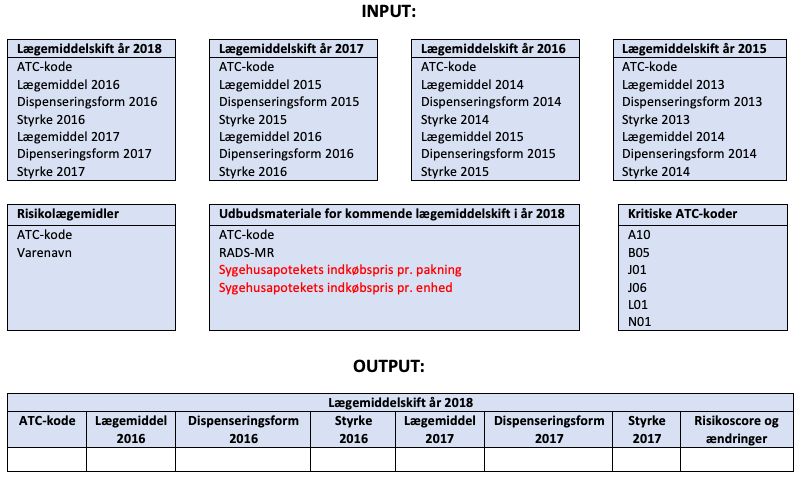
\includegraphics[width=1\textwidth]{billeder/InputOutput.png} 
	\caption{Input og output}
	\label{fig:InputOutput}  
\end{figure}



%Data er indsamlet af Amgros og omhandler de aftaler som er indgået i forbindelse med Amgrosudbud. Dette omfatter både forlængelser af allerede eksisterende kontrakter samt ændringer forårsaget af kontraktskift. Sygehusapoteket Region Nordjylland (SRN) udtrækker data fra sygehusapoteksportalen og sorterer i forhold til relevans. Den data der udtrækkes fra sygehusapoteksportalen indeholder alle de aftaler som er indgået, hvorfor det er nødvendigt at sortere indhold for den pågældende udbudsperiode. Denne sortering varetages af en ansat på SRN som udarbejder skiftelister ud fra proceduren, der er beskrevet i Appendiks \ref{cha:AppD} nummer \ref{item:Skiftelister}, hvorefter disse skiftelister sendes ud til de forskellige ATC-ansvarlige, som sortere ud fra ATC-koder i forhold til deres område.

%I dette projekt tages der udgangspunkt i data fra skiftelisterne, som bygger på skiftelister udarbejdet for lægemiddelskift i år 2014-2015(n=231), 2015-2016 (n = 160), 2016-2017 (n=232) og 2017-2018 (n=247). Data indeholder oplysninger om lægemiddelnavn, dispenseringsform og styrke for det fortgående år samt året hvor skiftet skal implementeres. Skiftelisterne kombineres med udtræk fra sygehusapoteksportalen omkring andre forhold som sygehusapotekets indkøbspris per enhed (SAIP/enhed) og oplysninger om hvorvidt lægemiddel er indeholdt i Medicinrådets behandlingsvejledning, hvor der anvendes en deterministisk metode til at matche data. Dette kombineres yderligere med data fra Amgros omhandlende risikolægemidler\fxnote{Overvej om det skal være	Risikosituationslægemidler fra pro.medicin i stedet} og indsamlet data fra SRN omkring kritiske ATC-koder.



%Data er indsamlet af Amgros og Sygehusapoteket Region Nordjylland (SRN) og omhandler lægemiddelskift i år 2018. Data fra Amgros omhandler oplysninger om lægemiddelskiftet foretaget fra år 2017 til 2018. Yderligere har Amgros udarbejdet et dokument over risikolægemidler, som fremgår af Appendiks \ref{cha:AppD}. Risikolægemidler er lægemidler som er særligt risikofyldte hvis disse ender i restordre, da erstatninger er svære at finde samt risikoen for fejl øges ved erstatning. Data fra SRN omhandler de udbud af lægemidler Amgros foretog inden et eventuelt kontraktskift for år 2018. 
%Udover dette har SRN ligeledes indsamlet de problemstillinger der har været vedrørende Amgrosskift siden år 2012.  





%Første trin omhandler identificering af problemer som systemet skal løse, herunder data som systemet skal arbejde på og tilgængelige ressourcer~\citep{Ligeza2006}. Det andet trin er omhandler identificering af nøglekoncepter samt relationer mellem disse som f.eks. typer af data, informationsstrøm og underliggende stukturer. Tredje trin involverer forståelse, beskrivelse og formalisering af problemet og hvordan løsninger findes. Denne proces bør omfatte verificering af systemet. Det fjerde trin har til formål at implementere den formaliseret viden i et program. Det sidste trin omfatter test ved validering af regler og implementeringen.~\citep{Ligeza2006}


\section{Risikofaktorer og vægtning}
Risikofaktorer er udvalgt ud fra den nuværende vurdering af ATC-ansvarlige medarbejdere, som fremgår af Appendiks~\ref{cha:AppD} punktnummer \ref{item:ATC-ansvarlig}. Litteratur som beskriver ændringer i forskellige faktorer som har ledt til medicineringsfejl i klinikken som følge af lægemiddelskift, hvilket fremgår af Afsnit \ref{sec:ProblemLaeg}. Dokumenterede ATC-koder af SRN, som har ledt til problemstillinger vedrørende lægemiddelskift og derfor anses som kritiske~\citep{SRN}. Lægemidler, der overvåges særligt af Amgros, som er risikofyldte, hvis de ender i restordre på grund af f.eks. leveringesvigt. Liste over risikolægemidler fremgår af Appendiks~\ref{cha:AppD} punktnummer \ref{item:Risikolaegemidler}. Risikofaktorerne er efter udvælgelsen vægtet af en ekspert inden for området, hvoraf en vægtning på 1 anses som værende af mindre betydning for implementering af lægemiddelskift og 5 anses som værende af stor betydning. Risikofaktorer, vægtning og begrundelse for valg fremgår af Tabel \ref{table:features}.

\begin{longtable}{p{3.5cm}| p{1cm} | p{9.5cm}}
	\caption{Risikofaktorer}
	\label{table:features} \\
\cellcolor[HTML]{C0C0C0} {\textbf{Risikofaktor}} & \cellcolor[HTML]{C0C0C0} {\textbf{Vægt}}& \cellcolor[HTML]{C0C0C0} {\textbf{Begrundelse}}  \\ \hline
\textbf{Navn} & 1 & Den hyppigste årsag til medicineringsfejl ved generisk substitution er ordinering af det forkerte lægemiddel, hvilket typisk skyldes at lægemidlets navn lignede og/eller havde et svært navn~\citep{Hakonsen2010}. \\  \hline 
\textbf{Look-a-like} & 2 & Look-a-like har påvist at kunne prædisponeres til medicineringsfejl~\citep{Wittich2014}. Dette kan have patientsikkerhedsmæssige konsekvenser, hvis f.eks. smertestillende panodil forveksles med plendil til behandling af forhøjet blodtryk ~\citep{DanskSelskabforPatientsikkerhed2009}.\\  \hline 
\textbf{Dispenseringsform} & 2 & Dispenseringsform giver anledning til medicineringsfejl i forbindelse med ordination~\citep{Agrawal2009}. Ved ordination af det forkerte lægemiddel, grundet navneforveksling, kan dette give anledning til fejl i dispenseringsform~\citep{DanskSelskabforPatientsikkerhed2009}, hvilket har en betydning for virkningen af lægemidlet.
\\ \hline 
\textbf{Styrke} & 2 & Styrke kan medføre medicineringsfejl ved ordination ved f.eks. forkert styrkeberegning~\citep{Agrawal2009}, hvorfor det er vigtigt at være opmærksom på  ændring i styrke for at undgå beregningsfejl og patienten får en højere eller lavere styrke end ordineret.\\ \hline
\textbf{Risikolægemidler} & 3 & Disse overvåges særligt af Amgros, da de er kritiske hvis de ender i restordre, hvorfor det anbefales at have disse på lager til 8 uger. Yderligere kræver nogle af disse lægemidler et ekstra personalemæssigt ressourcetræk i forbindelse med skift og er i øget risiko for utilsigtede hændelser, som beskrevet i Appendiks ~\ref{cha:AppD}, nummer \ref{item:Risikolaegemidler}  \\ \hline 
\textbf{ATC-grupper} & 5 & ATC-grupper som, A10, B05, J01, J06, L01 og N01, har givet anledning til problemstillinger vedrørende lægemiddelskift og er derfor defineret af SRN som kritiske \citep{SRN}.
%står for en stor andel af udgifterne til sygehusmedicin. Over halvdelen af den samlede omsætning er f.eks. til gruppe L som blandt andet inkluderer behandlingen af kræftmedicin, gigtbehandling og sklerose. Andre eksempler er HIV-behandling, øjenbehandlingen og infektioner som er omkostningsfulde.~\citep{Rapport2009}. Da der ofte er store besparelser at opnå ved disse lægemidler skal implementering foregå hurtigt.
 \\ \hline 
\textbf{Medicinråd} & 5 & Lægemidler som indgår i medicinrådets behandlingsvejledninger er lægemidler som er besluttet at anvendes som standardbehandling~\citep{Medicinradet2018}. Disse vurderes i forhold til effekt, eksisterende behandling og pris~\citep{Medicinradet2018}. For lægemidler som indgår i Medicinrådet er der ofte mange penge og spare, hvorfor disse skal implementeres hurtigt. \\ \hline 
%\textbf{Pris} &  2 & Pris er vigtigt i forhold til at opnå besparelser. Det skal ligeledes vægtes om det kan betale sig at skifte et lægemiddel med mindre besparelse, da udskiftningen kan få store betydninger for klinikken i forhold til arbejdsgangen og i værste tilfælde medføre patientsikkerhedsmæssige konsekvenser. [KILDE, AMGROS] \textcolor{blue}{Det er endnu ikke besluttet, hvordan denne faktor skal indgå i algoritmen.} \\ \hline
    \end{longtable}

\section{Præprocessering}
Præprocessering af data er nødvendigt, da data er tekstbaseret og indskrevet manuelt og derfor ikke sammenligneligt. Det er forskelligt om data er skrevet med majuskel eller minuskel, hvorfor det er valgt at ændre alt data til minuskel. Ligeledes er forkortelser udskrevet og tegnsætning fjernet for at gøre data generaliserbar. 

Det er valgt at antage at lægemiddelnavne er ens, hvis deres præfiks er uændret, hvorfor suffiks er fjernet. Lægemidler med ens præfiks, men forskellig suffiks, kan dog have anderledes dispenseringsform eller styrke. Dette vil opdages i forbindelse med sammenligning af dispenseringsform og styrke. 

For dispenseringsformer antages det at filmovertrukne tabelletter er det samme som tabelletter og hvis dispenseringsform ikke er angivet er denne uændret.

\section{Design}
Risikovurdering er designet ud fra IF-THEN statements som danner grundlag for risikovurderingen. Hvis et statement er sandt beregnes en risikoscore ud fra Ligning \ref{equ:risikoscore}. Derudover beskrives der, hvad der danner grundlag for den beregnede risikoscore.

\begin{equation}  \label{equ:risikoscore}
Riskoscore = \frac{\mbox{\textit{Summen af vægten af ikke matchende features}}}{\mbox{\textit{Summen af alle vægtede features}}} * 100
\end{equation}


%\begin{equation} \label{eq1}
%\begin{split}
%Risikoscore = lægemiddelnavn + ligende lægemiddelnavn + dispenseringsform \\ 
%+ styrke + medicnråd + risikolægemiddel + kritisk ATC-kode \\
%+ pris
%\end{split}
%\end{equation}

\section{Implementering}
Det er valgt at implementere koden i NetBeans, som er et Integrated Development Environment (IDE) til java. For at kunne håndtere Microsoft dokumenter blev Java Excel API (JExcelApi) og Apache POI tilføjet til biblioteket. Tegnsættet blev ændret til ISO-8859-15 i NetBeans IDE for at kunne håndtere æ, ø og å. 

\section{Evaluering}
Systemet evalueres for at undersøge anvendeligheden af systemet. Dette gøres i et gruppeinterview med ATC-ansvarlige medarbejdere på SRN, som systemet er tiltænkt. Med udgangspunkt i outputtet, foretages evaluering af risikoscore samt begrundelse for denne score. Ligeledes   diskuteres forbedringer til systemet med henblik på videre udvikling af systemet. 

\chapter{Resultat}



